\documentclass{chi2011}
\input ../Resources/latex/std-macros
\usepackage{times}
\usepackage{xspace}
\usepackage[usenames,dvipsnames]{color}
\usepackage{booktabs}
\usepackage{colortbl}
\usepackage{amsmath}
\usepackage{graphicx}


\newcommand{\system}{Colorific\xspace}
\newcommand{\graycol}{\cellcolor[gray]{0.7}}

\begin{document}

% --- Copyright notice ---
\conferenceinfo{UIST'09}{October 4-7, 2009, Victoria, British Columbia, Canada}
\CopyrightYear{2009}
\crdata{978-1-60558-745-5/09/10}

% Uncomment the following line to hide the copyright notice
 \toappear{}
% ------------------------


\title{\system: A Mixed Initiative Model Colorizer}

\numberofauthors{2}
\author{
  \alignauthor Chinmay Kulkarni\\
    \affaddr{Stanford University HCI Group}\\
    \affaddr{Stanford, CA 94305}\\
    \email{chinmay@cs.stanford.edu}
  \alignauthor Julie Fortuna\\
    \affaddr{Stanford University HCI Group}\\
    \affaddr{Stanford, CA 94305}\\
    \email{jfortuna@stanford.edu}
}

\maketitle

\abstract
Is it possible to automatically create a color palette relevant to a topic? Could such a palette be used to guide color choices while visualizing data? We present \system, a tool that automatically identifies relevant colors and palettes for a broad range of topics, and a mixed-initiative tool that allows tweaking of generated palettes. Evaluation shows \system verified that \system generates an acceptable set of relevant colors.
\classification{H5.2 [Information interfaces and presentation]:
User Interfaces. - Graphical user interfaces.}

\keywords{Information visualization, colors, mixed initiative}

\tolerance=400 
  % makes some lines with lots of white space, but 	
  % tends to prevent words from sticking out in the margin

\section{INTRODUCTION}
\input introduction.tex

\section{RELATED WORK}
\input related.tex
\section{SYSTEM DESCRIPTION}
\input algorithm.tex
\section{SYSTEM EVALUATION}
\input evaluation.tex
\section{DISCUSSION}
\input discussion.tex
\section{SCENARIO: DESIGNING WITH COLORIFIC}
Let's follow David, as he makes a bar chart of the number of games won by a selection of Pac-10 football teams. 
David begins creating his chart in Microsoft Excel, but Excel colors each bar from a pre-defined set of colors. David wants to color each bar a representative color for the team. He loads \system to see what colors it suggests. Based on the nominal values he is plotting, such as the Stanford Cardinal and the Cal Bears \system automatically generates a selection of four potential palettes he can choose from and plots his data values on a bar chart. David selects one automatically generated palette, which looks almost the way he wants it. However, after seeing the results in context, he thinks the Cal Bears bar should be gold instead of blue. He clicks on the bar and is presented with a selection of other \system generated colors for the Cal Bears, as well as a color picker that allows him to tweak \system colors or select his own. 

\begin{figure}[htb]
\label{screenshot}
\scalebox{0.25}{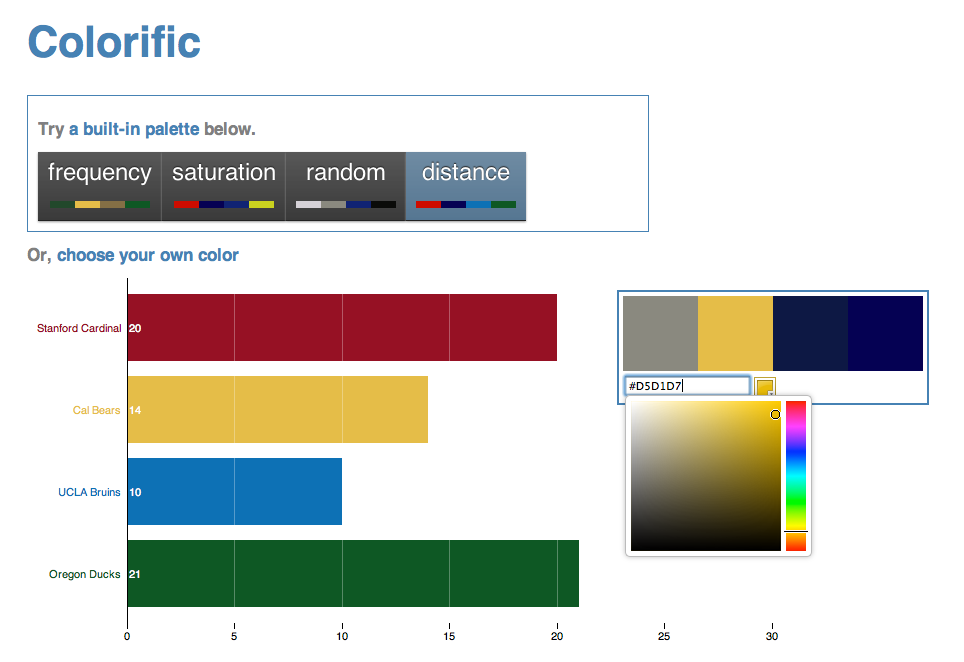
\includegraphics{colorific_screenshot.png}}
\caption{Screenshot of \system.}
\end{figure}
\section{DESIGN SPACE}
\system provides one point in the space of many data visualization tools. We summarize the decisions we made using the design space in Figure 4. 

\begin{figure}[htb]
\label{design-space}
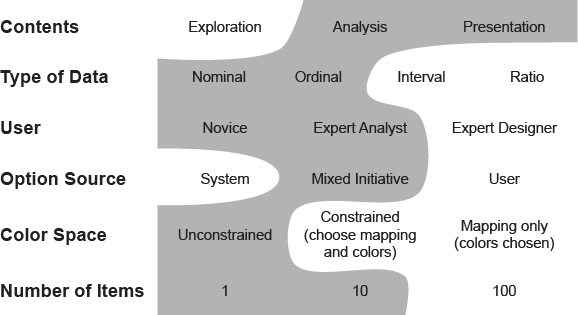
\includegraphics[scale=0.9]{design_space.png}
\caption{\system design space. Implemented choices in gray.}
\end{figure}
\textbf{Design Context} We believe having the right colors for a visualization help most in the analysis and the presentation stages. Therefore, \system provides no support for the ETL (extract-transform-load) stage of data visualization. However, these stages may also benefit, and perhaps guide the analyst in deciding which data is interesting.

\textbf{User} \system is meant for non-expert users and possibly expert analysts. For novices, the main advantage of \system are pre-made palettes, which already have desirable properties, but can be tweaked and edited. For experts, \system's main advantage is saving time. 

\textbf{Color Space} \system considers any color from the LAB space an equally viable candidate. Where the color space is constrained, this is not the case (for example, in printing techniques where only a few colors are available). While \system can be extended to these applications, by constraining the clustering algorithm, we defer this to future work.
\section{CONCLUSION}
This paper presents a mixed initiative model for color choice in information visualization. The insight driving our research is that topically-related images contain topically relevant colors. 
Going forward, it is promising to integrate \system in to a general visualization/analysis tool such as Excel. Another problem worth addressing is finding appropriate colors in a constrained color space, and improving built-in palettes offered by \system based on data from our Mechanical Turk experiments. 
%\section{ACKNOWLEDGMENTS} 
%We would like to thank Jeff Heer, Scott Klemmer and Jesse Cirimele for their valuable thoughts and encouragement, the Stanford HCI group for funding our Mechanical Turk experiments, and the participants in our in-person pilots and online experiments.

\bibliographystyle{abbrv}

\bibliography{../Resources/references/color-refs,../Resources/references/recommender-refs}
\end{document}
